\documentclass[border = 10pt]{standalone}
%% Preamble %%
\usepackage{tikz}
\usepackage{newpxtext,newpxmath}            % upright Greek

\renewcommand{\familydefault}{\sfdefault}   % sans sarif
\usepackage{mathastext}                     % common look for text and maths

\usetikzlibrary{positioning, quotes, calc, arrows.meta, shapes, math}

\tikzset{
  every edge quotes/.style = {fill = white},
  > = {Stealth[length = 1.5mm]},       % Stealth arrowheads
  shorten > = 1pt,                     % Both ends of the arrows (ie, variances and covariances)       
  shorten < = 1pt,                     %    end 1pt short of the node
  manifest/.style = {draw, inner sep = 3pt, align = center, 
    minimum width = 1cm, minimum height = 0.85cm},
  latent/.style = {manifest, ellipse},
  residual/.style n args = {3}{inner sep = #1, minimum size = #2, #3},   % #3   draw
  residual/.default = {0}{0}{},                                
  constant/.style = {draw, inner sep = 1pt, minimum size = 5mm,
    regular polygon, regular polygon sides = 3},
  regression/.style = {->, shorten < = 0pt, inner sep = 1.5pt},
  covariance/.style n args = {3}{<->, inner sep = 1.5pt, bend #1 = #2, looseness = #3},
                        % #1  bend "right" or "left"; #2  bend angle; #3  looseness
  variance/.style n args = {3}{covariance = {#1}{#2}{#3}, inner sep = 0.5pt},
  interaction/.style = {-{Stealth[sep = 1pt, length = 1.5mm] . Circle[length = 4pt]},
    shorten > = -2pt},
  group/.style = {inner sep = 2pt, align = center, minimum width = 15mm, minimum height = 5mm}
}


\def \gap {2cm}                                     % gap between dependents
\def \dependent {Life\\Satisfaction}                % dependent variable
\def \groups {No strategy, Discussion, Exercise}    % group names

\begin{document}
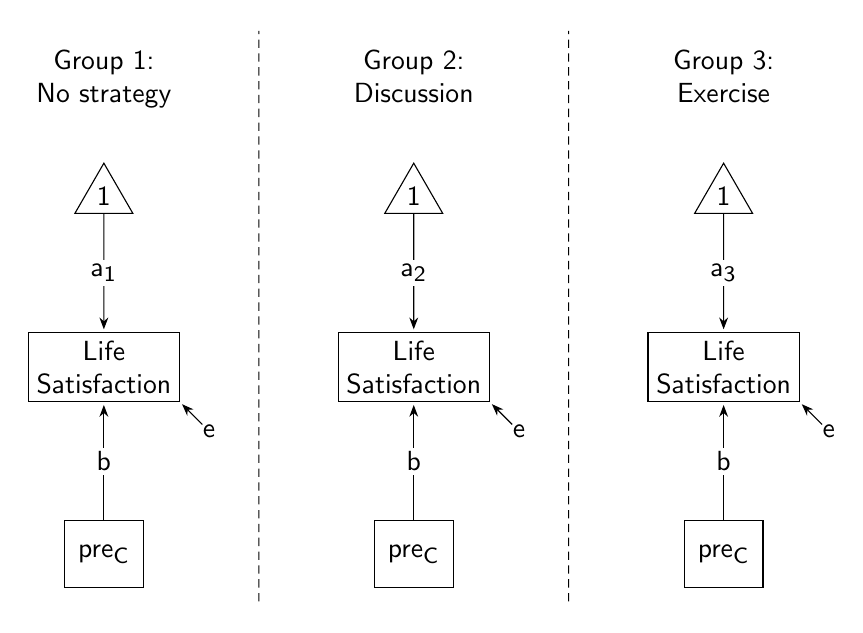
\begin{tikzpicture}

%% Dependents
\node [manifest] (y1) {\dependent};
\node [manifest] (y2) [right = \gap of y1] {\dependent};
\node [manifest] (y3) [right = \gap of y2] {\dependent};

\foreach \j [count = \i, remember = \i as \lasti] in \groups {  
  %% Residuals
  \node [residual] (e\i) [below right = 4mm of y\i] {e};
  \path [regression] (e\i) edge (y\i.south east);

  %% Covariates
  \node [manifest] (pre\i) [below = 1.5cm of y\i] {pre$_C$};
  \path [regression] (pre\i) edge ["b"] (y\i);

  %% Means
  \node [constant] (const) [above = 1.5cm of y\i] {1};
  \path [regression] (const) edge ["a$_\i$"] (y\i);

  %% Groups
  \node [group] (gp\i) [above = 1.5cm of const, anchor = north] {Group \i:\\\j};
  
  %% Separators
  \ifnum \i > 1
    \coordinate (m1) at ($(pre\i.south) !0.5! (pre\lasti.south)$);
    \coordinate (m2) at ($(gp\i.north) !0.5! (gp\lasti.north)$); 
    \draw [densely dashed] ($(m1) !-0.2cm! (m2)$) -- ($(m2) !-0.2cm! (m1)$);
  \fi  
}

\end{tikzpicture}
\end{document}